Bei dieser Option hätte lediglich eine weitere externe API für Statistance entwickelt werden mpssen, welches auf die Schnittstellen der Drittsysteme zugreift und das Ergebnis anschließend direkt dem Aufrufer (Applikation von Statistance) zurückgibt. Dabei hätten die Daten nicht nochmal in einer separaten Datenbank abgespeichert werden müssen. Die Abbildung \ref{fig:Entwicklung einer API ohne eigene Datenbank} veranschaulicht die Architektur dieser Option.

\begin{figure}[!h]
\centering
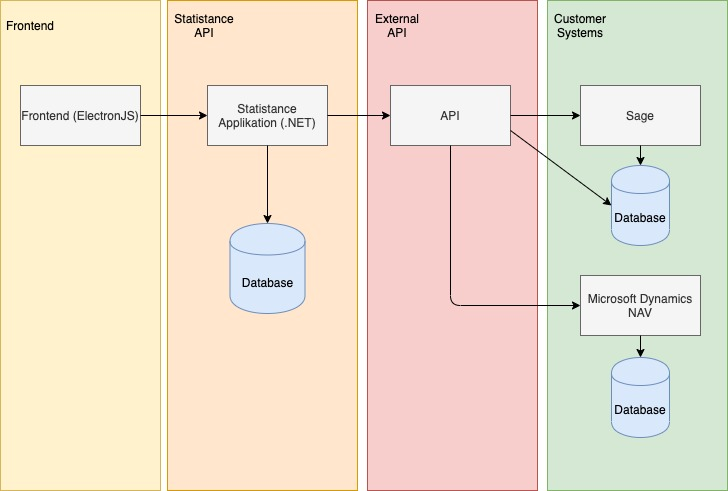
\includegraphics[width=15cm]{images/0x_implementation_possibilities/opt1.jpg}
\caption{Entwicklung einer API ohne eigene Datenbank}
\label{fig:Entwicklung einer API ohne eigene Datenbank}
\end{figure}

Bei dieser Option ergaben sich einige Vor- und Nachteile.\\
Der größte Vorteil dieser Option basierte auf der Einfachheit der Lösung mit einer geringen Komplexität. Daraus hätte sich eine schnelle Entwicklung ergeben, da keine zusätzlichen Services entwickelt und keine weiteren Infrastrukturkomponenten bereitgestellt werden müssen. Dementsprechend war diese Option auch am kostengünstigsten und am schnellstmöglichen umzusetzen. Allerdings ergaben sich hierbei auch einige Nachteile. Der größte Nachteil war die schlechte Skalierung dieses Systems. Bei steigenden Anforderungen und erhöhter Nachfrage, wird es immer schwieriger, weitere Systeme ohne viel zusätzlichen Aufwand bedienen zu können. Da die Daten nicht in einer separaten Datenbank abgespeichert werden, kann es bei der Antwort (Response) zu starken Verzögerungen bei Massendaten kommen, da diese gegebenfalls erst transformiert werden müssen, bevor sie an den Aufrufer geliefert werden können. Falls bei der Bearbeitung Fehler auftreten, müsste der gesamte Prozess nochmal von vorne angestoßen werden, da die Daten nicht zwischengespeichert werden. 